\section{Ejercicio 1}

Peso asignado: 8.

\subsection{Problema}

Se tiene un entero que representa el presupuesto con el que se cuenta y un
arreglo de enteros donde cada elemento representa el precio de un paquete. Se
quiere conocer cuál es la maxima cantidad de dinero que pueda ser gastada
comprando alguna combinación de paquetes, sin pasarse del presupuesto
determinado.

La complejidad temporal del algoritmo debe ser \ord($N \times 2^{N / 2}$) donde
$N$ es la cantidad de paquetes.

\subsection{Solución propuesta}

El algoritmo propuesto para resolver este problema es generar todas las
combinaciones de paquetes mediante \textit{Backtracking} y de ellas elegir la
mayor que no supere al presupuesto dado. La complejidad temporal de este
algoritmo es \ord($2^N$), lo cual no cumple con los requerimientos, pero esta
comlejidad puede ser fácilmente alcanzable utilizando la técnica conocida como
\textit{Meet in the middle}.

Esta técnica consiste en separar en dos mitades la entrada del problema, correr
el algortimo de backtraking en cada una y procesar los dos resultados
inteligentemente para llegar a una solución. Debe hacerse enfoque en encontrar
alguna manera en la que se pueda llegar a un resultado sin que el algoritmo
acabe teniendo en una complejidad igual a la de un \textit{Backtracking} puro.
Deben analizarse las salidas de las mitades de manera provechosa.

Posteriormente en este informe se demostrará por qué este algoritmo cumple con
los requerimientos de complejidad temporal para este ejercicio.

Es necesario aclarar que el algoritmo es válido cuando el vector de entrada
tiene al menos un elemento y el presupuesto es mayor o igual a cero.

La solución llevada a cabo consiste entonces en separar el arreglo en dos
mitades $A$ y $B$, a cada una se le aplica un algoritmo que devuelve un arreglo
que contiene todas las sumas posibles de los elementos de la entrada. Esto deja
dos arreglos, llamémoslos $S_A$ y $S_B$. $S_A$ contiene todas las posibles
combinaciones de sumas de paquetes de $A$ y $S_B$ las de $B$.

Lo que se hace en este momento es ordenar crecientemente alguno de los dos y
recorrer linealmente el otro. Se ordena $S_B$, por ejemplo, y se recorren todos
los elementos de $S_A$. Sea $p$ el entero de la entrada que representa el
presupuesto, para cada elemento $i$ de $S_A$ se busca en $S_B$ el máximo valor
$j$ tal que $i + j \leq p$. Es importante que la búsqueda en $S_B$ sea a través
de búsqueda binaria.

De todos los valores $i,j$ se toman los que sumados sea el máximo, siempre
cumpliendo que $i + j \leq p$, y ese es el resultado.

\bigskip

\begin{algorithm}[H]
	\caption{Algoritmo principal}
	\Input{Arreglo $paquetes$ de números enteros, entero $p$}
	\Output{Devuelve la máxima suma de paquetes tal que sea menor o igual a $p$}
    $n \gets paquetes$.tamaño() \;
	$mitad \gets n / 2$ \;

	$sumas_1 \gets posiblesSumas(paquetes[0..mitad))$ \;
	$sumas_2 \gets posiblesSumas(paquetes[mitad..n])$ \;

	ordenar($sumas_2$) \;

	$maxDonas \gets 0$ \;
	\For{$paq$ en $sumas_1$} {
		\If {$paq \leq p$} {
			$sum \gets paq + busqBin(sumas_2, p - paq)$ \;
			\If {$sum > maxDonas$} {
				$maxDonas \gets sum$ \;
			}
		}
	}

	\If {$sumas_1$.tamaño() $== 0  \land sumas_2[1] \leq p$} {
		$maxDonas \gets sumas_2[1]$ \;
	}

	\Return $maxDonas$ \;
\end{algorithm}

Puede apreciarse al final del algoritmo una estructura de decisión. Su propósito
es simplemente salvar el caso en el que el arreglo de entrada tiene un único
elemento, lo que lleva a que al dividir el arreglo en dos quede la primer mitad
sin elementos por lo cual nunca se entra en la estructura de repetición. Esto es
porque si el arreglo es de largo impar el elemento extra queda en la segunda
mitad, que al ser sobre la cual se hace la búsqueda binaria es levemente
conveniente que el arreglo mas largo de las dos mitades sea ese. Como se sabe
que el arreglo tiene al menos un elemento, si las sumas de la primer mitad no
tiene elementos entonces la sumas de la segunda tiene dos elementos: 0 y el
único elemento del arreglo original.

\subsection{Correctitud}

Para demostrar que el algoritmo es correcto, es decir que la salida se
corresponde con lo requerido, debe demostrarse que el resultado del algoritmo es
la máxima suma de elementos del arreglo de entrada tal que es menor o igual al
entero que representa el presupuesto.

Lo primero que realiza el algoritmo es dividir en mitades el arreglo de entrada
y aplicar fuerza bruta sobre cada uno para conocer todas combinaciones de sumas
de los elementos de cada arreglo. Esto deja entonces los arreglos que
previamente fueron nombrados como $S_A$ y $S_B$.

Cada elemento en estos arreglos representa intrínsecamente una combinación de
elementos de $A$ y de $B$, ya que cada elemento de $S_A$ y $S_B$ es calculado
mediante decidir si cada elemento de $A$ y $B$, respectivamente, forma parte de
la suma o no.

\begin{figure}[H]
	\centering
	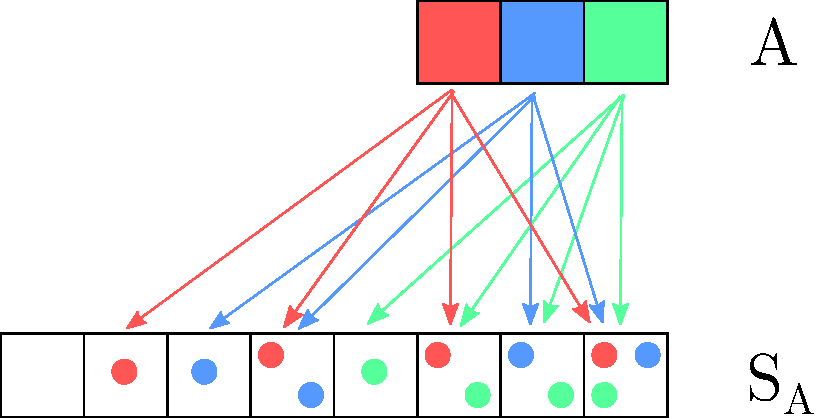
\includegraphics[scale=0.6]{imagenes/ex1_example1.pdf}
	\caption{Ejemplo de los posibles conjuntos de un arreglo.}
	\label{ej1:fig:combinations}
\end{figure}

En otras palabras, cada elemento de $S_A$ y $S_B$ es una suma de uno de los
$2^{N / 2}$ conjuntos de elementos que pueden formarse de $A$ y $B$
respectivamente, donde cada conjunto es distinto al anterior, por lo que se
exploran todos los conjuntos posibles de $A$ y de $B$.

Entonces si se tiene separados todos los conjuntos posibles de $A$ y todos los
de $B$, se tiene todos los conjuntos posibles del arreglo original. Mediante la
suma de ambos valores se obtiene un elemento que representa una combinación
única de los elementos del arreglo original. Esto no quiere decir que los
valores sean distintos, de hecho es muy probable que se repitan como en el
siguiente ejemplo

\begin{figure}[H]
	\centering
	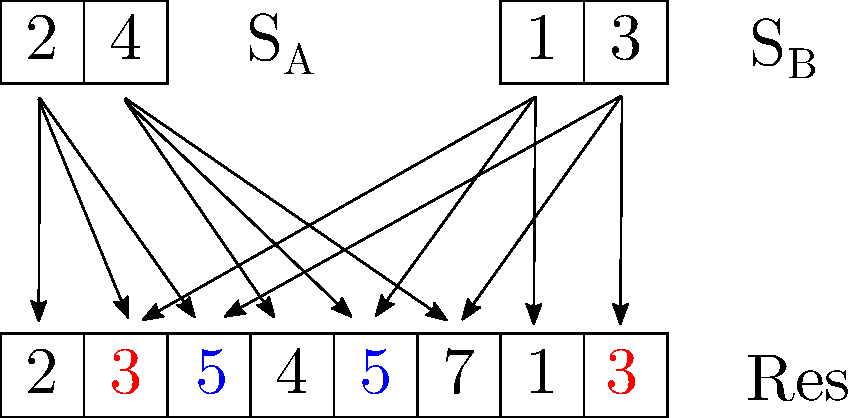
\includegraphics[scale=0.6]{imagenes/ex1_example2.pdf}
	\caption{Ejemplo de posible repetición de valores sumando conjuntos
	distintos.}
	\label{ej1:fig:value_repetition}
\end{figure}


pero como puede observarse cada uno representa una combinación de elementos
distinta.

De esta forma se tienen calculadas las sumas de todas la posibles combinaciones
del arreglo de entrada, por lo que solo resta buscar las que cumplan ser menor o
igual al presupuesto y entre ellas la máxima.


\subsection{Complejidad teórica}

Se divide el arreglo de entrada en dos, lo cual tiene un costo lineal. Ahora
estos arreglos tienen un tamaño de $\frac{n}{2}$. A cada uno de ellos se le
calcula, a través de un algoritmo de \textit{Backtracking} por fuerza bruta,
todas las posibles sumas de sus elementos. Como fue hablado anteriormente, es
equivalente a formar todos los posibles subconjuntos lo cual tiene costo
$\ord(2^{largo(arreglo)})$  y como el tamaño de los arreglos es de
$\frac{n}{2}$, el costo es de $\ord(2^{\frac{n}{2}})$.

Una vez hecho esto se ordena uno de los dos arreglos. Esto cuesta
$\ord(largo(arreglo) \times log(largo(arreglo)))$ lo cual en este caso es
$\ord(2^{\frac{n}{2}} \times log(2^{\frac{n}{2}}))$ que a su vez es
$\ord(2^{\frac{n}{2}} \times n)$.

Para finalizar se recorre linealmente el arreglo no ordenado realizando para
cada uno de sus elementos una búsqueda binaria sobre el arreglo ordenado, y
quedándose con el mayor. Recorrer el arreglo no ordenado cuesta
$\ord(2^{\frac{n}{2}})$ y hacer una búsqueda en el arreglo ordenado
$\ord(log(2^{\frac{n}{2}}))$ que es equivalente a $\ord(n)$ por lo que el costo
de este recorrido es $\ord(2^{\frac{n}{2}} \times n)$.

La complejidad final es entonces
$\ord(2^{\frac{n}{2}} + 2^{\frac{n}{2}} \times n + 2^{\frac{n}{2}} \times n)$
$ = \ord(2^{\frac{n}{2}} \times n)$.

\subsection{Casos de prueba}

Luego de comprobar que el algoritmo se comportaba de manera correcta con
respecto a los tests de la cátedra fueron generadas otras instancias de prueba
con el fin de cubrir todos los posibles casos del problema.

\begin{itemize}
\item Caso borde con un único elemento. Es necesario para comprobar que el
algoritmo se comporta adecuadamente no sólo al ser una cantidad impar de
elementos sino al dejar una de las mitades sin elementos, lo cual podría traer
problemas al momento de hacer los recorridos.
\item Caso en que todos los elementos superan el presupuesto. Debería devolver
0. Es importante ya que es el valor predeterminado en caso en que todas las
opciones fueran descartadas.
\item Caso en que el resultado es el menor elemento del arreglo. El motivo de
esto es para corroborar la buena funcionalidad de la busqueda binaria, resulta
ser uno de los casos borde para el cual hay que tener cuidado a la hora de
implementar la búsqueda.
\item Casos normales en los que no se comprueba un caso borde en especial.
\end{itemize}